% Options for packages loaded elsewhere
% Options for packages loaded elsewhere
\PassOptionsToPackage{unicode}{hyperref}
\PassOptionsToPackage{hyphens}{url}
\PassOptionsToPackage{dvipsnames,svgnames,x11names}{xcolor}
%
\documentclass[
  letterpaper,
  DIV=11,
  numbers=noendperiod]{scrreprt}
\usepackage{xcolor}
\usepackage{amsmath,amssymb}
\setcounter{secnumdepth}{5}
\usepackage{iftex}
\ifPDFTeX
  \usepackage[T1]{fontenc}
  \usepackage[utf8]{inputenc}
  \usepackage{textcomp} % provide euro and other symbols
\else % if luatex or xetex
  \usepackage{unicode-math} % this also loads fontspec
  \defaultfontfeatures{Scale=MatchLowercase}
  \defaultfontfeatures[\rmfamily]{Ligatures=TeX,Scale=1}
\fi
\usepackage{lmodern}
\ifPDFTeX\else
  % xetex/luatex font selection
\fi
% Use upquote if available, for straight quotes in verbatim environments
\IfFileExists{upquote.sty}{\usepackage{upquote}}{}
\IfFileExists{microtype.sty}{% use microtype if available
  \usepackage[]{microtype}
  \UseMicrotypeSet[protrusion]{basicmath} % disable protrusion for tt fonts
}{}
\makeatletter
\@ifundefined{KOMAClassName}{% if non-KOMA class
  \IfFileExists{parskip.sty}{%
    \usepackage{parskip}
  }{% else
    \setlength{\parindent}{0pt}
    \setlength{\parskip}{6pt plus 2pt minus 1pt}}
}{% if KOMA class
  \KOMAoptions{parskip=half}}
\makeatother
% Make \paragraph and \subparagraph free-standing
\makeatletter
\ifx\paragraph\undefined\else
  \let\oldparagraph\paragraph
  \renewcommand{\paragraph}{
    \@ifstar
      \xxxParagraphStar
      \xxxParagraphNoStar
  }
  \newcommand{\xxxParagraphStar}[1]{\oldparagraph*{#1}\mbox{}}
  \newcommand{\xxxParagraphNoStar}[1]{\oldparagraph{#1}\mbox{}}
\fi
\ifx\subparagraph\undefined\else
  \let\oldsubparagraph\subparagraph
  \renewcommand{\subparagraph}{
    \@ifstar
      \xxxSubParagraphStar
      \xxxSubParagraphNoStar
  }
  \newcommand{\xxxSubParagraphStar}[1]{\oldsubparagraph*{#1}\mbox{}}
  \newcommand{\xxxSubParagraphNoStar}[1]{\oldsubparagraph{#1}\mbox{}}
\fi
\makeatother


\usepackage{longtable,booktabs,array}
\usepackage{calc} % for calculating minipage widths
% Correct order of tables after \paragraph or \subparagraph
\usepackage{etoolbox}
\makeatletter
\patchcmd\longtable{\par}{\if@noskipsec\mbox{}\fi\par}{}{}
\makeatother
% Allow footnotes in longtable head/foot
\IfFileExists{footnotehyper.sty}{\usepackage{footnotehyper}}{\usepackage{footnote}}
\makesavenoteenv{longtable}
\usepackage{graphicx}
\makeatletter
\newsavebox\pandoc@box
\newcommand*\pandocbounded[1]{% scales image to fit in text height/width
  \sbox\pandoc@box{#1}%
  \Gscale@div\@tempa{\textheight}{\dimexpr\ht\pandoc@box+\dp\pandoc@box\relax}%
  \Gscale@div\@tempb{\linewidth}{\wd\pandoc@box}%
  \ifdim\@tempb\p@<\@tempa\p@\let\@tempa\@tempb\fi% select the smaller of both
  \ifdim\@tempa\p@<\p@\scalebox{\@tempa}{\usebox\pandoc@box}%
  \else\usebox{\pandoc@box}%
  \fi%
}
% Set default figure placement to htbp
\def\fps@figure{htbp}
\makeatother





\setlength{\emergencystretch}{3em} % prevent overfull lines

\providecommand{\tightlist}{%
  \setlength{\itemsep}{0pt}\setlength{\parskip}{0pt}}



 


\KOMAoption{captions}{tableheading}
\makeatletter
\@ifpackageloaded{bookmark}{}{\usepackage{bookmark}}
\makeatother
\makeatletter
\@ifpackageloaded{caption}{}{\usepackage{caption}}
\AtBeginDocument{%
\ifdefined\contentsname
  \renewcommand*\contentsname{Table of contents}
\else
  \newcommand\contentsname{Table of contents}
\fi
\ifdefined\listfigurename
  \renewcommand*\listfigurename{List of Figures}
\else
  \newcommand\listfigurename{List of Figures}
\fi
\ifdefined\listtablename
  \renewcommand*\listtablename{List of Tables}
\else
  \newcommand\listtablename{List of Tables}
\fi
\ifdefined\figurename
  \renewcommand*\figurename{Figure}
\else
  \newcommand\figurename{Figure}
\fi
\ifdefined\tablename
  \renewcommand*\tablename{Table}
\else
  \newcommand\tablename{Table}
\fi
}
\@ifpackageloaded{float}{}{\usepackage{float}}
\floatstyle{ruled}
\@ifundefined{c@chapter}{\newfloat{codelisting}{h}{lop}}{\newfloat{codelisting}{h}{lop}[chapter]}
\floatname{codelisting}{Listing}
\newcommand*\listoflistings{\listof{codelisting}{List of Listings}}
\makeatother
\makeatletter
\makeatother
\makeatletter
\@ifpackageloaded{caption}{}{\usepackage{caption}}
\@ifpackageloaded{subcaption}{}{\usepackage{subcaption}}
\makeatother
\usepackage{bookmark}
\IfFileExists{xurl.sty}{\usepackage{xurl}}{} % add URL line breaks if available
\urlstyle{same}
\hypersetup{
  pdftitle={My Personal Reviews},
  pdfauthor={Mineva Azzahra},
  colorlinks=true,
  linkcolor={blue},
  filecolor={Maroon},
  citecolor={Blue},
  urlcolor={Blue},
  pdfcreator={LaTeX via pandoc}}


\title{My Personal Reviews}
\usepackage{etoolbox}
\makeatletter
\providecommand{\subtitle}[1]{% add subtitle to \maketitle
  \apptocmd{\@title}{\par {\large #1 \par}}{}{}
}
\makeatother
\subtitle{Portfolio Asesmen II-2100 KIPP}
\author{Mineva Azzahra}
\date{2025-10-15}
\begin{document}
\maketitle

\renewcommand*\contentsname{Table of contents}
{
\hypersetup{linkcolor=}
\setcounter{tocdepth}{2}
\tableofcontents
}

\bookmarksetup{startatroot}

\chapter*{Hai!}\label{hai}
\addcontentsline{toc}{chapter}{Hai!}

\markboth{Hai!}{Hai!}

\begin{figure}[H]

{\centering \includegraphics[width=9.5\linewidth,height=\textheight,keepaspectratio]{images/AZRL.png}

}

\caption{About Me}

\end{figure}%

\begin{center}\rule{0.5\linewidth}{0.5pt}\end{center}

\section*{Selamat Datang! ₍\^{}. .\^{}₎⟆}\label{selamat-datang-.-.}
\addcontentsline{toc}{section}{Selamat Datang! ₍\^{}. .\^{}₎⟆}

\markright{Selamat Datang! ₍\^{}. .\^{}₎⟆}

Saya \textbf{Mineva Azzahra}, seorang mahasiswi Sistem dan Teknologi
Informasi dari Bandung.

\begin{center}\rule{0.5\linewidth}{0.5pt}\end{center}

\section*{Bingkai Berpikir: Penumpang atau
Pengemudi?}\label{bingkai-berpikir-penumpang-atau-pengemudi}
\addcontentsline{toc}{section}{Bingkai Berpikir: Penumpang atau
Pengemudi?}

\markright{Bingkai Berpikir: Penumpang atau Pengemudi?}

Dalam hidup, ada dua cara memandang perjalanan: sebagai penumpang yang
pasrah mengikuti arus, atau sebagai pengemudi yang sadar memegang
kendali. Konsep psikologis tentang \emph{Locus of Control} menyadarkan
saya bahwa keyakinan akan kendali diri bukanlah takdir, melainkan sebuah
pilihan sadar. Saya belajar bahwa merasa berdaya atau tidak berdaya
sering kali dimulai dari cara kita membingkai cerita kita sendiri.
Apakah hidup ini sesuatu yang \emph{terjadi pada saya}, atau sesuatu
yang \emph{saya jalani}?

\bookmarksetup{startatroot}

\chapter{\textgreater{} All About Me}\label{all-about-me}

\begin{figure}[H]

{\centering 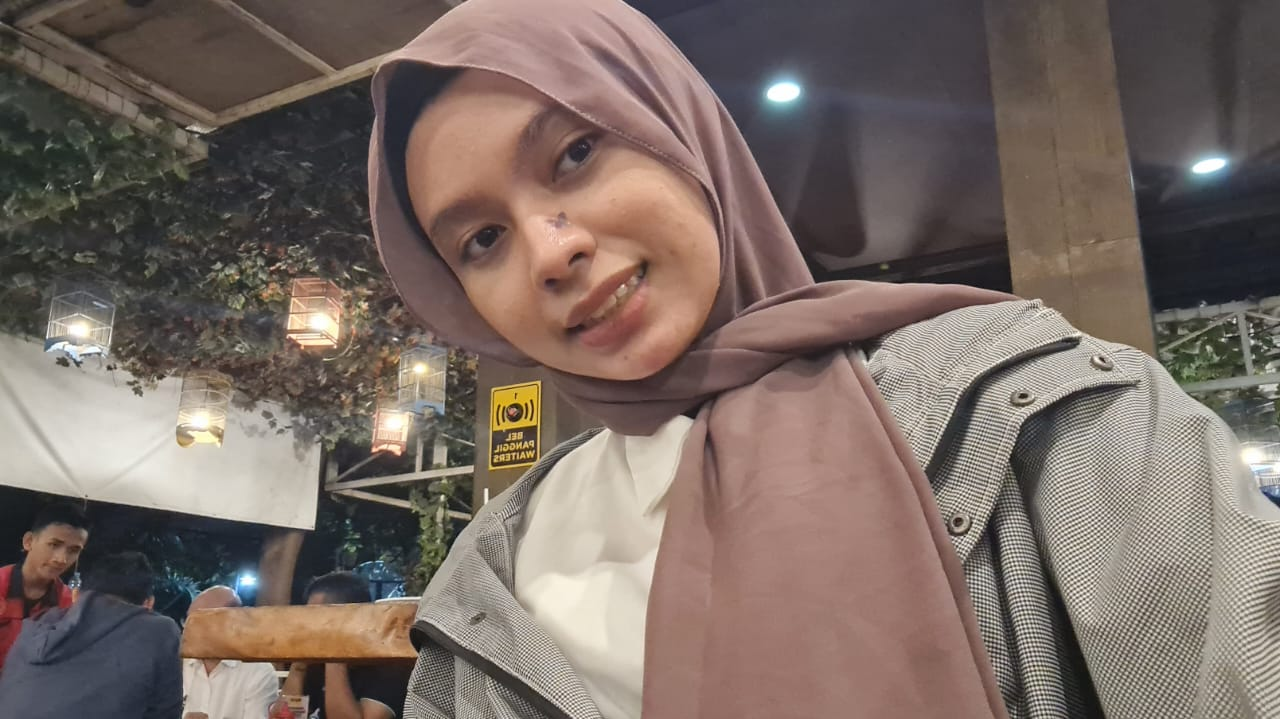
\includegraphics[width=1\linewidth,height=\textheight,keepaspectratio]{images/mi.jpeg}

}

\caption{Hello}

\end{figure}%

\begin{quote}
I am both the sun and the moon, therefore, I complete myself.
\end{quote}

\begin{center}\rule{0.5\linewidth}{0.5pt}\end{center}

\section{Selamat Datang!}\label{selamat-datang}

---to Mineva's page

Saya \textbf{\emph{Mineva Azzahra}} dan saya berasal dari
\textbf{\emph{Bandung}} (warga lokal sekitar ITB). Saya berasal dari
jurusan Sistem dan Teknologi Informasi. Mahasiswa yang percaya bahwa
setiap orang adalah sistem yang unik, dan saya bersemangat untuk
mempelajari \emph{source code} yang membentuk interaksi antarmanusia.
Jurusan ini bagi saya bukan hanya tentang belajar teknologi, tetapi juga
menjadi semacam \emph{panduan pengguna} untuk memahami dunia yang
semakin kompleks di sekitar saya.

\emph{Saya menemukan bahwa efektivitas terbaik lahir dari lingkungan
yang terstruktur, namun inovasi paling signifikan justru muncul dari
kebebasan berpikir yang tidak terikat apapun!}

\section{Sedikit Perkenalan Lagi}\label{sedikit-perkenalan-lagi}

\begin{itemize}
\tightlist
\item
  \textbf{Panggilan:} Minep/Eva/Neo
\item
  \textbf{Bahasa yang Didukung:} Indonesia (Native), Inggris (Enough),
  Sunda (Native).
\item
  \textbf{Waktu Aktif:} Paling optimal di sore dan malam hari.
\end{itemize}

\section{Fokus Pengembangan Diri}\label{fokus-pengembangan-diri}

\begin{itemize}
\tightlist
\item
  \textbf{Peningkatan Keterampilan}: Meningkatkan kompetensi di bidang
  desain (khususnya UI/UX dan desain grafis), terus memperdalam keahlian
  yang relevan dengan Sistem dan Teknologi Informasi.
\end{itemize}

\bookmarksetup{startatroot}

\chapter{\textgreater{} My Songs for You}\label{my-songs-for-you}

\begin{quote}
\emph{Songs I have personal connection with.}
\end{quote}

\section{To Life Itself?}\label{to-life-itself}

\section{Sebelah Mata}\label{sebelah-mata}

\url{https://youtu.be/u5aHyZV0CTI?si=zNwUnuZnOY9taS2E}

\begin{quote}
Tapi sebelah mataku yang lain menyadari

Gelap adalah teman setia

Dari waktu-waktu yang hilang
\end{quote}

Bukan genre lagu yang biasanya saya nikmati, tapi atmosfernya sangat
menghanyutkan. Entah mengapa ini jadi salah satu lagu yang paling sering
saya putar di tahun 2024. Jadi pengingat bahwa tidak semua hal harus
selalu ceria dan penuh semangat.

\section{For Myself}\label{for-myself}

\section{In My Mouth}\label{in-my-mouth}

\url{https://youtu.be/cIi4SxZ0IC8?si=EeUQOrJCeDpnrkRK}

\begin{quote}
I don't feel like I can be anything more than this

I don't really want to be anything more than this

I just wanna be whatever you want me to be

I don't wanna have a soul
\end{quote}

Lagu ini salah satu tipe musik yang saya sukai dan ada kenangan
tersendiri. Lagunya menyajikan ekspresi emosi yang sangat jujur dan
mentah, sulit diungkapkan dengan kata-kata biasa. Perpaduan antara lirik
yang intens tentang kehancuran diri, dan keinginan akan koneksi, dengan
musik yang abrasif, menciptakan pengalaman katarsis bagi saya sendiri.

Mendengarkan ini mungkin seperti ada di pusat badai. Tapi intinya, ada
keheningan. Semua orang bisa melewati kekacauan dalam keadaan utuh.

\emph{Kamu pusatnya, bukan korbannya}.

\section{For My Beloveds}\label{for-my-beloveds}

\subsection{Credo Quia Absurdum}\label{credo-quia-absurdum}

\url{https://youtu.be/1X9GzzGerLk?si=nfli4dUuje805mxc}

\begin{quote}
Through the torii of a weathered shrine, I pass

There's no light but I'm dazzled nonetheless

I feel I might drown in the winter sea,

and it feels so gentle.
\end{quote}

Lagu ber-subgenre favorit saya. Bassnya asik.

Seperti pengingat bahwa kenyamanan bisa muncul dari hal-hal yang tidak
selalu hangat atau terang. Ada orang yang menemukan tenangnya di tengah
keramaian, ada juga yang baru bisa bernapas saat dunia terasa hening.
Ada ketenangan yang hanya bisa ditemukan lewat orang-orang yang kita
sayangi, bukan karena mereka menghapus kekosongan, tapi karena mereka
membuatnya terasa lebih hangat.

Tenggelam bukan selalu berarti hilang, kadang justru cara kita kembali
merasa utuh, dan kehadiran seseorang juga bisa jadi tempat pulang.

\bookmarksetup{startatroot}

\chapter{\textgreater{} My Stories for You}\label{my-stories-for-you}

\begin{quote}
\emph{Is the story old? yes. Is it still a problem? yes.}
\end{quote}

\subsection{\texorpdfstring{\textbf{Standar Prosedur untuk Tertinggal di
Lobi}}{Standar Prosedur untuk Tertinggal di Lobi}}\label{standar-prosedur-untuk-tertinggal-di-lobi}

Di dalam mobil, aku tubuh kecil yang menempel di jendela. Ada
suara-suara yang ramai dan akrab, terdengar seperti radio dari ruangan
lain, begitu dekat sekaligus jauh. Aku tidak ikut mendengarkan,
dua-duanya, aku tidak mau dan aku tidak bisa. Mataku sibuk melacak
garis-garis emas yang dibuat matahari saat menembus debu di udara, atau
menonton pohon-pohon yang nampak seperti mimpi buruk yang aku sukai. Aku
ada di antara mereka, tapi duniaku sendiri ada di balik kaca, sunyi dan
penuh dengan hal-hal kecil yang hanya aku yang melihat.

Lalu kami berhenti di sebuah tempat yang besar dan terbuka di dekat
Borobudur. Suara-suara itu menjauh, sibuk berbicara dengan orang di
balik meja kayu yang tinggi. Aku ditinggalkan sendiri untuk sesaat,
mataku terpaku pada sebuah patung dari batu di dekat kolam kecil. Aku
mau membawanya pulang, harusnya boleh.

Aku mendengar langkah kaki mereka yang menjauh, kembali ke pintu tempat
kami masuk. Salah satu dari mereka menoleh sekilas, tapi tatapannya
lewat begitu saja. Lalu sebuah pertanyaan kecil yang aneh muncul:
\emph{bagaimana kalau aku tidak ikut?} Jadi, aku tidak bergerak. Aku
hanya melangkah ke samping, bahkan tidak bersembunyi, hanya melangkah
beberapa langkah kecil. Tidak lama, aku melihat mobil itu menyala dan
perlahan pergi, membawa semua keramaian itu bersamanya.

Setelah mobil itu hilang, rasanya luar biasa? Seperti baru saja
menemukan sebuah tombol rahasia, dan dengan menekannya, suara statis
yang ramai di kepalaku, akhirnya mati. Yang tersisa bukanlah sepi,
melainkan sebuah keheningan yang jernih. Satu-satunya suara adalah
gemericik air dari kolam. Aku berjalan mendekati patung batu di kolam
itu, menyentuh kepalanya yang dingin. Tidak ada yang menelepon, tidak
ada yang panik. Untuk pertama kalinya, aku tidak hanya dipaksa mendengar
dan aku bisa memilih suara apa yang ingin kudengarkan. Dan aku memilih
ini.

⋆⋅☆⋅⋆ ──────

\textbf{\emph{Saya belajar bahwa inti dari perjalanan ini bukanlah
tentang pasrah pada alurnya, melainkan tentang mengambil tanggung jawab
penuh atas arah yang saya tuju. Masa depan mungkin terasa abstrak,
tetapi tindakan yang saya ambil hari ini sangatlah nyata. Karena itu,
kegigihan saat menghadapi kesulitan, rasa ingin tahu untuk terus
belajar, dan kemampuan beradaptasi saat rencana berubah menjadi prinsip
utama saya. Ini bukan soal menjadi sempurna, tapi soal kesadaran bahwa
sayalah yang bertanggung jawab untuk membangun jalan saya sendiri,
langkah demi langkah}}

\bookmarksetup{startatroot}

\chapter{\textgreater{} My SHAPE}\label{my-shape}

\begin{quote}
\textbf{Tujuan:} Merangkum rancangan diri agar saya dapat belajar,
berkarya, dan bertumbuh secara paling selaras dengan panggilan dan
pengalaman unik saya. Dokumen ini berfungsi sebagai acuan aksi untuk 90
hari ke depan dan seterusnya.
\end{quote}

\begin{center}\rule{0.5\linewidth}{0.5pt}\end{center}

\section{Ringkasan}\label{ringkasan}

\textbf{Peran Inti:} Pemecah masalah teknis yang berfokus pada sisi
manusia dari teknologi.

\textbf{Misi:} Mengintegrasikan analisis sistem yang logis dengan
pemahaman empati terhadap pengguna, untuk merancang dan menciptakan
solusi teknologi yang fungsional sekaligus humanis.

\textbf{Kekuatan Utama:} Pemikiran sistematis, analisis kebutuhan
pengguna, dasar-dasar desain antarmuka (UI/UX), riset mandiri, dan
kemampuan belajar yang adaptif.

\textbf{Dampak yang Dituju:} Produk digital yang intuitif, solusi
teknologi yang menjawab masalah nyata pengguna, dan kontribusi pada tim
yang menjembatani antara aspek teknis dan pengalaman pengguna.

\textbf{Peta SHAPE (singkat):}

\begin{itemize}
\tightlist
\item
  \textbf{S --- Panggilan Inti:} Analisis \& Sintesis, Empati,
  Integritas, Otonomi.
\item
  \textbf{H --- Minat \& Gairah:} Desain yang berpusat pada pengguna
  (\emph{user-centered design}); psikologi kognitif dalam interaksi
  manusia-komputer; penerapan teknologi untuk pemecahan masalah;
  mempelajari bagaimana narasi membentuk pengalaman emosional.
\item
  \textbf{A --- Abilities (Kemampuan):} Analisis \& perancangan sistem,
  dasar-dasar pemrograman (Python/Java), prototyping UI/UX (Figma),
  riset \& analisis data, komunikasi teknis tertulis.
\item
  \textbf{P --- Personality (Gaya Kerja):} Metodis \& terstruktur,
  mandiri \& proaktif (\emph{self-driven}), analitis, menghargai
  profesionalisme dan fokus pada tujuan bersama.
\item
  \textbf{E --- Experiences (Pengalaman Pembentuk):} Pengalaman formatif
  tentang pentingnya agensi dan pengambilan keputusan sadar; proyek
  akademis di STI; pembelajaran mandiri di bidang desain; analisis media
  (musik/film) untuk memahami emosi pengguna.
\end{itemize}

\begin{center}\rule{0.5\linewidth}{0.5pt}\end{center}

\section{S --- Panggilan Inti (Core
Calling)}\label{s-panggilan-inti-core-calling}

\begin{itemize}
\tightlist
\item
  \textbf{Analisis \& Sintesis:} Kemampuan untuk mengurai masalah
  kompleks menjadi komponen logis dan menyatukannya kembali menjadi
  sebuah solusi yang koheren.
\item
  \textbf{Empati:} Dorongan untuk memahami ``mengapa'' di balik tindakan
  pengguna; menempatkan diri pada posisi mereka untuk menemukan titik
  masalah yang sebenarnya.
\item
  \textbf{Integritas \& Otonomi:} Kebutuhan untuk bekerja secara mandiri
  dengan standar tinggi, mengambil tanggung jawab penuh atas hasil kerja
  dan proses pengambilan keputusan.
\end{itemize}

\begin{center}\rule{0.5\linewidth}{0.5pt}\end{center}

\section{H --- Heart (Minat Profesional \& Gairah
Intelektual)}\label{h-heart-minat-profesional-gairah-intelektual}

\begin{itemize}
\tightlist
\item
  \textbf{Desain Berpusat pada Pengguna:} Ketertarikan mendalam pada
  proses menciptakan produk yang tidak hanya berfungsi baik, tetapi juga
  mudah dan menyenangkan untuk digunakan.
\item
  \textbf{Psikologi dalam Teknologi:} Gairah untuk mempelajari bagaimana
  pikiran manusia bekerja dan menerapkan wawasan tersebut untuk
  membangun interaksi digital yang lebih baik.
\item
  \textbf{Pemecahan Masalah:} Antusiasme dalam menghadapi tantangan
  teknis atau konseptual dan merancang solusi yang efektif dan efisien.
\item
  \textbf{Analisis Naratif:} Minat dalam menganalisis bagaimana cerita,
  musik, dan media lain dapat membangkitkan emosi, sebagai dasar untuk
  merancang pengalaman yang lebih kaya.
\end{itemize}

\begin{center}\rule{0.5\linewidth}{0.5pt}\end{center}

\section{A --- Abilities (Kemampuan
Andal)}\label{a-abilities-kemampuan-andal}

\begin{itemize}
\tightlist
\item
  \textbf{Analisis Sistem \& Proses:} Mampu memetakan alur kerja,
  mengidentifikasi \emph{bottlenecks}, dan merancang proses yang lebih
  efisien.
\item
  \textbf{Dasar-dasar Desain UI/UX:} Menguasai prinsip-prinsip desain
  antarmuka dan pengalaman pengguna, serta mampu membuat prototipe awal
  menggunakan Figma.
\item
  \textbf{Riset \& Pembelajaran Mandiri:} Terampil dalam mencari,
  menyaring, dan mensintesis informasi baru secara mandiri untuk
  mempelajari teknologi atau metodologi baru.
\item
  \textbf{Komunikasi Tertulis:} Mampu menyusun dokumen teknis, laporan
  analisis, dan argumen desain secara jelas dan terstruktur.
\end{itemize}

\begin{center}\rule{0.5\linewidth}{0.5pt}\end{center}

\section{P --- Personality (Gaya Kerja
Profesional)}\label{p-personality-gaya-kerja-profesional}

\begin{itemize}
\tightlist
\item
  \textbf{Metodis \& Terstruktur:} Bekerja dengan pendekatan
  langkah-demi-langkah, memastikan setiap detail dipertimbangkan.
\item
  \textbf{Mandiri \& Proaktif:} Tidak menunggu instruksi; aktif mencari
  masalah untuk dipecahkan dan mengambil inisiatif untuk memulai.
\item
  \textbf{Fokus pada Solusi:} Ketika menghadapi masalah, orientasi utama
  adalah menemukan solusi praktis, bukan terjebak dalam diskusi yang
  tidak produktif.
\item
  \textbf{Kolaborator yang Profesional:} Menghargai komunikasi yang
  jelas, tepat sasaran, dan menjaga hubungan kerja yang saling
  menghormati.
\end{itemize}

\begin{center}\rule{0.5\linewidth}{0.5pt}\end{center}

\section{E --- Experiences (Pengalaman
Pembentuk)}\label{e-experiences-pengalaman-pembentuk}

\begin{itemize}
\tightlist
\item
  \textbf{Proyek Akademis STI:} Melatih kemampuan analisis, kerja tim,
  dan manajemen proyek dalam lingkungan yang terstruktur dan
  berorientasi pada hasil.
\item
  \textbf{Pengambilan Keputusan Sadar:} Pengalaman pribadi yang
  mengajarkan pentingnya agensi dan keberanian dalam mengambil keputusan
  untuk menentukan arah, bahkan saat menghadapi ketidakpastian.
\item
  \textbf{Pembelajaran Desain Mandiri:} Proses belajar UI/UX secara
  otodidak yang membangun disiplin, rasa ingin tahu, dan portofolio
  awal.
\item
  \textbf{Analisis Media:} Kebiasaan menganalisis musik, film, dan
  cerita yang mengasah kepekaan terhadap emosi dan narasi, memberikan
  wawasan unik untuk memahami pengguna.
\end{itemize}

\begin{center}\rule{0.5\linewidth}{0.5pt}\end{center}

\section{Piagam Diri}\label{piagam-diri}

\textbf{Misi Profesional:} Menjadi jembatan antara dunia teknis dan
kebutuhan manusia, dengan merancang solusi teknologi yang didasari oleh
data, logika, dan empati yang mendalam.

\textbf{Nilai Inti:} Empati, Logika, Integritas, Pertumbuhan, Kualitas.

\textbf{Peran Ideal:} Analis Sistem, Desainer UX/UI, Peneliti Pengguna
(User Researcher).

\textbf{Kompas Keputusan:} (1) Apakah ini memecahkan masalah nyata bagi
pengguna? (2) Apakah solusinya logis dan efisien? (3) Apakah prosesnya
dilakukan dengan integritas? (4) Apakah ini memberikan ruang untuk
belajar dan bertumbuh?

\textbf{Janji Profesional:} Untuk selalu memulai dengan pertanyaan
``mengapa'', mendengarkan kebutuhan pengguna sebelum merancang solusi,
dan bertanggung jawab penuh atas kualitas hasil kerja.

\begin{center}\rule{0.5\linewidth}{0.5pt}\end{center}

\section{Narasi}\label{narasi}

Ketertarikan saya pada Sistem dan Teknologi Informasi lahir dari
keyakinan bahwa di balik setiap kerumitan, selalu ada pola yang bisa
ditemukan. Saya melihat dunia sebagai kumpulan sistem yang saling
terhubung dan menemukan kepuasan dalam mengurainya.

Di bangku kuliah, keyakinan itu semakin terasah. Saya belajar bahwa
merancang sistem yang baik bukan hanya tentang efisiensi kode, tetapi
tentang empati, kemampuan untuk memahami alur pikir pengguna. Saya
menemukan bahwa teknologi terbaik bukanlah yang paling rumit, melainkan
yang paling intuitif.

Namun, saya sadar bahwa tidak semua hal bisa diurai dengan logika.
Melalui tulisan dan musik, saya memahami spektrum emosi manusia yang
lebih kompleks, mengajarkan bahwa pemahaman utuh datang dari analisis
dan perenungan.

Ke depan, saya ingin terus berkarya di titik pertemuan antara analisis
sistem dan pengalaman manusia. Saya tidak hanya ingin membangun
aplikasi, tetapi merancang interaksi yang menghargai waktu dan perhatian
penggunanya. Baik melalui baris kode yang elegan atau tulisan yang
jujur, tujuan saya tetap sama: menciptakan ruang yang lebih sederhana
dan terfokus, agar kita bisa lebih mudah terhubung dengan apa yang
benar-benar penting.

\bookmarksetup{startatroot}

\chapter{\textgreater{} My Personal Reviews}\label{my-personal-reviews}

\begin{quote}
``Asik yah.''
\end{quote}

\begin{center}\rule{0.5\linewidth}{0.5pt}\end{center}

\subsection{1 --- All About Me}\label{all-about-me-1}

\begin{longtable}[]{@{}
  >{\raggedright\arraybackslash}p{(\linewidth - 4\tabcolsep) * \real{0.3000}}
  >{\centering\arraybackslash}p{(\linewidth - 4\tabcolsep) * \real{0.4000}}
  >{\raggedright\arraybackslash}p{(\linewidth - 4\tabcolsep) * \real{0.3000}}@{}}
\toprule\noalign{}
\begin{minipage}[b]{\linewidth}\raggedright
Kriteria
\end{minipage} & \begin{minipage}[b]{\linewidth}\centering
Nilai
\end{minipage} & \begin{minipage}[b]{\linewidth}\raggedright
Catatan Singkat
\end{minipage} \\
\midrule\noalign{}
\endhead
\bottomrule\noalign{}
\endlastfoot
\textbf{Orisinalitas} & 5 & Ide dan narasi sangat personal, mencerminkan
identitas unik penulis. \\
\textbf{Keterlibatan} & 4 & Gaya tulisan menarik, namun bisa lebih
diperkuat untuk membangun koneksi emosional yang lebih dalam. \\
\textbf{Humor} & 3 & Fokus pada nada reflektif dan serius; humor bukan
elemen utama dalam tulisan ini. \\
\textbf{Wawasan} & 5 & Menunjukkan kesadaran diri yang tinggi dan
koneksi yang jelas antara nilai pribadi dengan tujuan. \\
\end{longtable}

\textbf{Rata-rata : 4.25 (A)} \textbf{Komentar:} Fondasi yang sangat
kuat dengan narasi personal yang otentik. Refleksi diri yang ditampilkan
menunjukkan pemikiran yang matang.

\begin{center}\rule{0.5\linewidth}{0.5pt}\end{center}

\subsection{2 --- My Song for You}\label{my-song-for-you}

\begin{longtable}[]{@{}
  >{\raggedright\arraybackslash}p{(\linewidth - 4\tabcolsep) * \real{0.3000}}
  >{\centering\arraybackslash}p{(\linewidth - 4\tabcolsep) * \real{0.4000}}
  >{\raggedright\arraybackslash}p{(\linewidth - 4\tabcolsep) * \real{0.3000}}@{}}
\toprule\noalign{}
\begin{minipage}[b]{\linewidth}\raggedright
Kriteria
\end{minipage} & \begin{minipage}[b]{\linewidth}\centering
Nilai
\end{minipage} & \begin{minipage}[b]{\linewidth}\raggedright
Catatan Singkat
\end{minipage} \\
\midrule\noalign{}
\endhead
\bottomrule\noalign{}
\endlastfoot
\textbf{Orisinalitas} & 4 & Pilihan lagu unik dan interpretasi personal,
namun narasi bisa lebih diperkaya dengan konteks spesifik. \\
\textbf{Keterlibatan} & 4 & Mampu membawa pembaca ke dalam suasana
reflektif lagu-lagu yang dipilih. \\
\textbf{Humor} & 3 & Nada tulisan cenderung serius dan introspektif,
sesuai dengan tema lagu. \\
\textbf{Inspirasi} & 5 & Pesan penutup tentang ``menjadi pusat, bukan
korban'' sangat kuat dan inspiratif. \\
\end{longtable}

\textbf{Rata-rata : 4.00 (A)} \textbf{Komentar:} Berhasil menunjukkan
kedalaman emosional dan kemampuan untuk menarik makna personal dari
sebuah karya seni.

\begin{center}\rule{0.5\linewidth}{0.5pt}\end{center}

\subsection{3 --- My Stories for You}\label{my-stories-for-you-1}

\begin{longtable}[]{@{}
  >{\raggedright\arraybackslash}p{(\linewidth - 4\tabcolsep) * \real{0.3000}}
  >{\centering\arraybackslash}p{(\linewidth - 4\tabcolsep) * \real{0.4000}}
  >{\raggedright\arraybackslash}p{(\linewidth - 4\tabcolsep) * \real{0.3000}}@{}}
\toprule\noalign{}
\begin{minipage}[b]{\linewidth}\raggedright
Kriteria
\end{minipage} & \begin{minipage}[b]{\linewidth}\centering
Nilai
\end{minipage} & \begin{minipage}[b]{\linewidth}\raggedright
Catatan Singkat
\end{minipage} \\
\midrule\noalign{}
\endhead
\bottomrule\noalign{}
\endlastfoot
\textbf{Orisinalitas} & 5 & Gaya penceritaan sangat otentik dan unik,
menciptakan pengalaman membaca yang sangat personal. \\
\textbf{Keterlibatan} & 5 & Narasi ``show, don't tell'' dieksekusi
sempurna, sangat berhasil menarik pembaca ke dalam cerita. \\
\textbf{Pengembangan Narasi} & 5 & Struktur cerita dan refleksi sangat
solid; alur dan tempo penceritaan terkontrol dengan sangat baik. \\
\textbf{Inspirasi} & 5 & Pesan tentang agensi diri dan tanggung jawab
personal tersampaikan secara mendalam dan berkesan. \\
\end{longtable}

\textbf{Rata-rata : 5.00 (A+)} \textbf{Komentar:} Sebuah karya tulis
yang luar biasa. Matang secara naratif, emosional, dan filosofis. Titik
puncak dari seri ini.

\begin{center}\rule{0.5\linewidth}{0.5pt}\end{center}

\subsection{4 --- My SHAPE}\label{my-shape-1}

\begin{longtable}[]{@{}
  >{\raggedright\arraybackslash}p{(\linewidth - 4\tabcolsep) * \real{0.3000}}
  >{\centering\arraybackslash}p{(\linewidth - 4\tabcolsep) * \real{0.4000}}
  >{\raggedright\arraybackslash}p{(\linewidth - 4\tabcolsep) * \real{0.3000}}@{}}
\toprule\noalign{}
\begin{minipage}[b]{\linewidth}\raggedright
Kriteria
\end{minipage} & \begin{minipage}[b]{\linewidth}\centering
Nilai
\end{minipage} & \begin{minipage}[b]{\linewidth}\raggedright
Catatan Singkat
\end{minipage} \\
\midrule\noalign{}
\endhead
\bottomrule\noalign{}
\endlastfoot
\textbf{Orisinalitas} & 5 & Analisis terasa lahir dari refleksi nyata
dan pengalaman pribadi, bukan sekadar mengisi template. \\
\textbf{Keterlibatan} & 5 & Struktur yang logis dan benang merah yang
kuat membuat dokumen ini sangat menarik dan mudah diikuti. \\
\textbf{Keautentikan} & 4 & Sangat otentik, namun bisa diperkuat lagi
dengan contoh/bukti konkret dari pengalaman yang disebutkan. \\
\textbf{Inspirasi} & 5 & Bagian ``Piagam Diri'' dan ``Kompas Keputusan''
sangat inspiratif dan dapat ditindaklanjuti (\emph{actionable}). \\
\end{longtable}

\textbf{Rata-rata : 4.75 (A)} \textbf{Komentar:} Analisis diri yang
sangat komprehensif dan strategis. Berhasil mengubah refleksi menjadi
sebuah panduan kerja yang jelas.

\begin{center}\rule{0.5\linewidth}{0.5pt}\end{center}

\subsection{Rangkuman Nilai Akhir}\label{rangkuman-nilai-akhir}

\begin{longtable}[]{@{}lcl@{}}
\toprule\noalign{}
UTS & Rata-rata & Tingkat \\
\midrule\noalign{}
\endhead
\bottomrule\noalign{}
\endlastfoot
\textbf{UTS-1 All About Me} & 4.25 & A \\
\textbf{UTS-2 My Song for You} & 4.00 & A \\
\textbf{UTS-3 My Stories for You} & 5.00 & A+ \\
\textbf{UTS-4 My SHAPE} & 4.75 & A \\
\textbf{Rata-rata Keseluruhan} & \textbf{4.50 / 5.00 (A)} & \\
\end{longtable}

\begin{center}\rule{0.5\linewidth}{0.5pt}\end{center}

\subsection{Kesimpulan}\label{kesimpulan}

Seluruh karya pada repositori \emph{All About Me} menunjukkan
\textbf{perkembangan kepribadian dan refleksi diri yang konsisten,
cerdas, dan mendalam.} Setiap UTS memperlihatkan kematangan berpikir
serta keaslian ekspresi yang khas. Tulisan-tulisan Anda tidak hanya
memenuhi rubrik akademik, tetapi juga berhasil menjadi potret perjalanan
intelektual dan personal yang otentik.

\begin{quote}
\emph{``Menjadi reflektif bukan berarti berhenti, melainkan melangkah
dengan lebih sadar akan arah dan makna.''}
\end{quote}

\bookmarksetup{startatroot}

\chapter{UAS-1 My Concepts}\label{uas-1-my-concepts}

Mau hidup epik ? \href{lifestory.pdf}{Write your Life Story}

Apa itu berkonsep?

\url{https://youtu.be/QVfUlVBO80U?si=yM6q_rwV9rcDBbu7}

\bookmarksetup{startatroot}

\chapter{UAS-3 My Opinions}\label{uas-3-my-opinions}

SApa itu beropini? \href{BM\%20Opini.mp4}{Opini Berpengaruh}

Bagiamana menjaadi menarik? \href{./Interesting.mp4}{Menjadi Menarik}

\bookmarksetup{startatroot}

\chapter{UAS-3 My Innovations}\label{uas-3-my-innovations}

\bookmarksetup{startatroot}

\chapter{UAS-4 My Knowledge}\label{uas-4-my-knowledge}

Cara saya mengkomunikasikan sebuah pengatahuan sebagai petunjuk bagi
orang lain 1) saya tulis
\href{Rekomendasi\%20Presentasi\%20Efektif(Contoh\%20Makalah).pdf}{makalah
sebagai bahan utama} 2) lalu saya buat
\href{Contoh\%20Transkrip\%20Presentasi.pdf}{transkrip ucapan lisan} 3)
kemudian saya kembangkan
\href{Rekomendasi\%20Presentasi\%20(Contoh\%20Slides).pdf}{slide
pendukung trnsskrip} 4) lalu saya memproduksivideo audio visual
\url{https://youtu.be/ZbghfMvnPZc} \url{https://youtu.be/ZbghfMvnPZc}

\bookmarksetup{startatroot}

\chapter{UAS-5 My Professional
Reviews}\label{uas-5-my-professional-reviews}

Untuk melAkukan review, seperti pada
\href{../My_Personal_Reviews/Doc.5.Mengevaluasi-Esai-Berdasarkan-Rubrik.pdf}{pendekatan
AI}, kita membutuhkan rubrik

\bookmarksetup{startatroot}

\chapter{Summary}\label{summary}

In summary, this book has no content whatsoever.

\bookmarksetup{startatroot}

\chapter*{References}\label{references}
\addcontentsline{toc}{chapter}{References}

\markboth{References}{References}

\phantomsection\label{refs}




\end{document}
